% vim: set spell spelllang=en tw=100 et sw=4 sts=4 :

\documentclass{llncs}

% \usepackage{showframe}

\usepackage{times}
\usepackage{complexity}
\usepackage{hyperref}
\usepackage{microtype}
\usepackage{cleveref}                  % no need to type Figure etc
\usepackage{xcolor,colortbl}

\usepackage{todonotes}
\usepackage{booktabs}

% lncs style
\crefname{algocf}{Algorithm}{Algorithms}
\Crefname{algocf}{Algorithm}{Algorithms}
\crefname{figure}{Fig.}{Figs.}
\Crefname{figure}{Fig.}{Figs.}
\crefname{table}{Table}{Tables}
\Crefname{table}{Table}{Tables}
\crefname{proposition}{Proposition}{Propositions}
\Crefname{proposition}{Proposition}{Propositions}

\title{Portfolios of Subgraph Isomorphism Algorithms}

\author{
    Lars Kotthoff\inst{1}
    \and Ciaran McCreesh\thanks{This work was supported by the Engineering
        and Physical Sciences Research Council [grant number EP/K503058/1]}\inst{2}
    \and Christine Solnon\inst{3}}

\institute{
    University of British Columbia, Vancouver, Canada
    \and University of Glasgow, Glasgow, Scotland
    \and INSA-Lyon, LIRIS, UMR5205, F-69621, France}

\begin{document}

\maketitle

\begin{abstract}
Subgraph isomorphism is a computationally challenging problem with lots of important practical
applications, for example in computer vision, biochemistry, and model checking. There are a number
of state-of-the-art algorithms for solving it, each of which has its own performance
characteristics. As with many other hard problems, the single best choice of algorithm overall is
rarely the best algorithm for each instance. We develop a portfolio approach that leverages novel
features to characterise subgraph isomorphism problems to dynamically decide which algorithm to use
on a per-instance basis. We demonstrate significant performance improvements on a large set of hard
benchmark problems. In addition, we show how algorithm selection models can be leveraged to gain new
insights into what affects the performance of an algorithm.
\end{abstract}

\section{Introduction}

The subgraph isomorphism problem is to find an injective mapping from vertices of a small
\emph{pattern} graph to vertices of a large \emph{target} graph which preserves adjacency. This
\NP-complete problem has lots of important practical applications, for example in computer vision
\cite{cviu11,pr15}, biochemistry \cite{Giugno:2013}, and model checking \cite{Sevegnani:2015}. There
exist various exact algorithms, which have been compared on a large benchmark in
\cite{McCreesh:2015}. These experiments indicated that the single best algorithm depends on the CPU
time limit considered: for very small (resp. larger) CPU time limits, VF2 \cite{Cordella:2004}
(resp. the Glasgow algorithm \cite{McCreesh:2015}) has better success rates. Furthermore, they also
showed us that on an instance by instance basis, other algorithms may become better.

In this paper, we report experimental results on a larger set of 8 algorithms, including new
variants, and a larger benchmark. We show that 4 of these algorithms are single best algorithms,
depending on the CPU time limit considered, and that combining preprocessing with an algorithm
selection on an instance by instance basis allows us to achieve better overall performance than any
single algorithm.

\section{Definitions and notations}

A \emph{graph} $G=(N,E)$ consists of a \emph{node set} $N$ and an \emph{edge set} $E \subseteq N \times N$, where an edge $(u,u')$ is a couple of nodes. The number of neighbors of a node $u$ is the degree of $u$, $d^\circ(u)=\#\{ (u,u')\in E\}$. In this paper, we implicitely consider non directed graphs, such that $(u,u')\in E\Leftrightarrow (u',u)\in E$. The extension to directed graphs is rather straightforward, and all algorithms compared in this paper can handle directed graphs as well.
   
A \emph{subgraph isomorphism problem} between a pattern graph $G_p=(N_p,E_p)$ and a target graph $G_t=(N_t,E_t)$ consists in deciding whether $G_p$ is isomorphic to some subgraph of $G_t$. More precisely, the goal is to find an injective matching $f: N_p\rightarrow N_t$, that associates a different target node to each pattern node, and that preserves pattern edges, i.e., $\forall (u,u') \in E_p, (f(u),f(u')) \in E_t$.

Note that the subgraph is not necessarily induced so that two pattern nodes that are not linked by an edge may be matched to two target nodes which are linked by an edge. This problem is also called subgraph monomorphism or subgraph matching in the literature. 
%{\em Induced subgraph isomorphism} is a particular case of subgraph isomorphism such that the subgraph isomorphism function must also preserve target edges between matched nodes, i.e., 
%\[\forall (u,u') \in N_p^2, (u,u')\in E_p \Leftrightarrow(f(u),f(u')) \in E_t\]

In the following, we assume $G_p=(N_p,E_p)$ and $G_t=(N_t,E_t)$ to be the underlying instance of subgraph isomorphism problem. 
We also define $n_p = \# N_p$, $n_t = \# N_t$,  $e_p=\# E_p$, $e_t=\# E_t$, and $d_p$ and $d_t$ the maximal degrees of the graphs $G_p$ and $G_t$. 


\section{Subgraph isomorphism algorithms}

Subgraph isomorphism problems may be solved by a systematic exploration of the search space composed of all possible injective matchings from $N_p$ to $N_t$: starting from an empty matching, one incrementally extends a partial matching by matching a non matched pattern node to a non matched target node until either some edges are not matched by the current matching (the search must backtrack to a previous choice point and go on with another extension) or all pattern nodes have been matched (a solution has been found). To reduce the search space, this exhaustive exploration is combined with filtering techniques that aim at removing candidate couples of non matched pattern-target nodes $(u,v)\in N_p\times N_t$. Different filterings may be considered; some are stronger than others (they remove more candidate couples), but also have higher time complexities.

\paragraph{Filtering for subgraph isomorphism.}

Simple filterings basically propagate difference constraints (which ensure that the matching is injective) and edge constraints (which ensure that the matching preserves pattern edges): each time a pattern node $u\in N_p$ is matched with a target node $v\in N_t$, one removes every candidate couple $(u',v')\in N_p\times N_t$ such that either $v'=v$ (difference constraint) or $(u,u')$ is a pattern edge whereas $(v,v')$ is not a target edge (edge constraint). This simple filtering (called {\em Forward-Checking}) is very fast to achieve: in ${\cal O}(n_p)$ for difference constraints, and in ${\cal O}(d_p\cdot n_t)$ for edge constraints. It is used, for example, in McGregor's algorithm \cite{mcgregor79} and in VF2 \cite{Cordella:2004}.

R\'egin has introduced in \cite{regin} a stronger filtering for difference constraints, which ensures that all pattern nodes can be matched with different target nodes, all together. This filtering (called {\em AllDifferent Generalized Arc Consistency}) removes more candidate couples than when each difference contraint is propagated separately which Forward-Checking. However, it is also more time consuming as it is done in ${\cal O}(n_p^2\cdot n_t^2)$.

Various filterings have been introduced for edge constraints. Ullman \cite{ullman} has introduced a filtering which basically ensures that for each pattern edge $(u,u')\in E_p$ and each candidate couple $(u,v)\in N_p\times N_t$, there exists a candidate couple $(u',v')\in N_p\times N_t$ such that $(v,v')$ is a target edge. Candidate couples $(u,v)$ that do not satisfy this property are iteratively removed until a fixed point is reached. This filtering (called {\em Arc Consistency}) removes more candidate couples than Forward-Checking, but it is also more time consuming as it is done in ${\cal O}(e_p\cdot n_t^2)$ when using the algorithm AC4  \cite{MH86}.

A stronger filtering may be obtained by propagating edge constraints in a more global way, as proposed in \cite{LV02}. The idea is to check for each candidate couple $(u,v)\in N_p\times N_t$ that the number of pattern nodes adjacent to $u$ is smaller than or equal to the number of target nodes that are both adjacent to $v$ and that may be matched with nodes adjacent to $u$. This is done in ${\cal O}(n_p^2\cdot n_t^2)$. This idea has been generalized in \cite{Solnon:2010} where, for each candidate couple $(u,v)\in N_p\times N_t$, a redundant Local AllDifferent (LAD) constraint ensures that each neighbour of $u$ may be matched with a different neighbour of $v$. This is done in ${\cal O}(n_p\cdot n_t\cdot d_p^2\cdot d_t^2)$.

\paragraph{Propagation of invariant properties.}

Some filterings exploit invariant properties, {\em i.e.}, properties associated with nodes such that nodes may be matched only if they have compatible properties. A classical property is the degree: a pattern node $u\in N_p$ may be matched with a target node $v\in N_t$ only if $d^\circ(u)\leq d^\circ(v)$. This property is usually used at the beginning of the search to reduce the set of candidate couples to $\{(u,v)\in N_p\times N_t\;|\;d^\circ(u)\leq d^\circ(v)\}$.
Other examples of invariant properties are the number of cycles of length $k$ passing through the node, and the number of cliques of size $k$ containing the node, which must be smaller for a pattern node than for its matched target node.
Invariant properties may also be associated with couples of nodes. For example, the number of paths of length $k$ between two pattern nodes is smaller than or equal to the number of paths of length $k$ between the target nodes they may be matched with. 

These invariant properties are used, for example:
\begin{itemize}
\item  In \cite{battiti-mascia07}, to remove candidate couples $(u,v)\in N_p\times N_t$ such that the number of paths starting from  pattern node $u$ is greater than the number of paths starting from  target node $v$~;
\item In \cite{Audemard:2014} to generalize the LAD constraint proposed in \cite{Solnon:2010} so that it ensures that a subset of pattern nodes can be matched with all different compatible target nodes, where compatibility is defined with respect to invariant properties~;
\item In \cite{McCreesh:2015} to filter the set of candidate couples before starting the search.
\end{itemize}
In \cite{Audemard:2014} , the length of paths is not limited, and it is iteratively incremented until no more couple is removed. In \cite{battiti-mascia07} and \cite{McCreesh:2015},  algorithms are parameterized by the maximum path length considered when counting paths: Larger values for this parameter remove more candidate couples, but are also more time consuming. Experiments reported in \cite{battiti-mascia07} show us that the best setting depends on the instance considered, and that a portfolio running several randomized 
versions in time-sharing decreases the total CPU-time needed to find a solution for feasible instances. In experiments reported in \cite{McCreesh:2015}, this parameter has been set to 3, as this setting seemed to be a reasonable compromise.


\paragraph{Algorithms selected in our portfolio.}
We have selected a set of algorithms with complementary performance:
\begin{itemize}
\item VF2 \cite{Cordella:2004}, which performs a weak filtering so that it is especially fast on trivially satisfiable instances;
\item LAD \cite{Solnon:2010}, which combines two strong but expensive filtering techniques (AllDifferent Generalized Arc Consistency and LAD);
\item Glasgow \cite{McCreesh:2015}, which does expensive preprocessing based on path length
    invariant properties to generate additional constraints, followed by weaker filtering
    (forward-checking, and a heuristic AllDifferent propagator which can miss deletions) and
    conflict-directed backjumping during search.
\end{itemize}

\noindent The Glasgow algorithm has a parameter, which controls the lengths of paths used when
reasoning about non-adjacent vertices.  In experiments reported in \cite{McCreesh:2015}, the choice
of paths of length 3 was used as a reasonable compromise---longer paths lead to prohibitively
expensive preprocessing on larger, denser instances. This is often not the best choice on an
instance by instance basis: sometimes path-based reasoning gives no benefit at all, sometimes
considering only paths of length 2 suffices, occasionally paths of length 4 are helpful, and even
looking at paths of length 3 is relatively expensive on some graphs.

\begin{figure}[!ht]
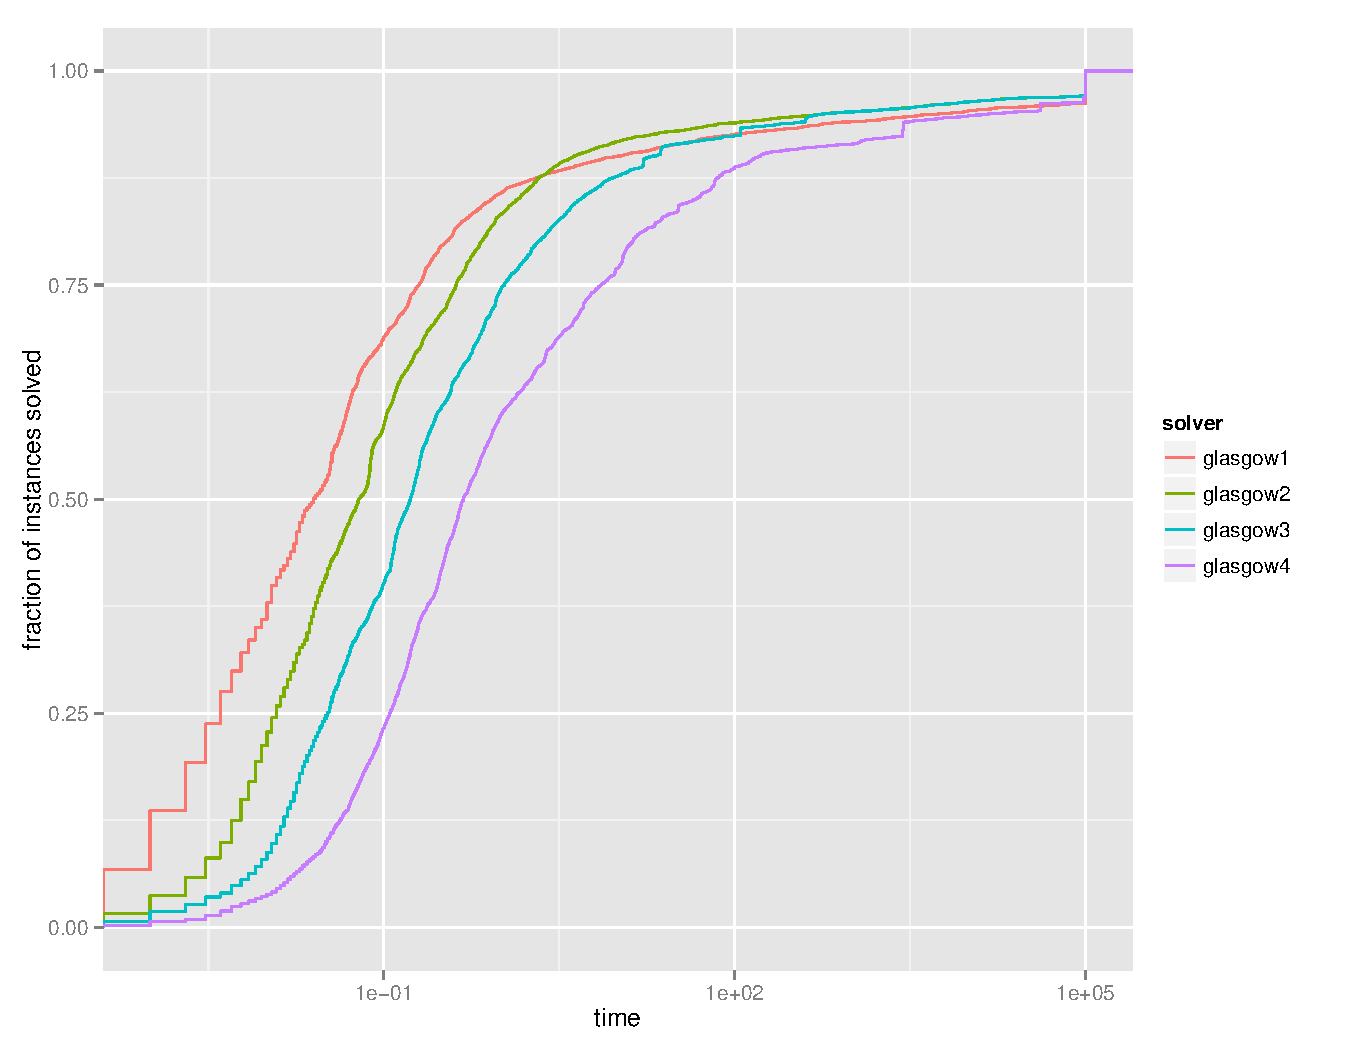
\includegraphics[width=\textwidth]{figures/ecdf-glasgow}
\caption{Empirical cumulative distribution function for the Glasgow algorithm
with path lengths 1, 2, 3, and 4.}
\label{fig:ecdf-glasgow}
\end{figure}

Figure~\ref{fig:ecdf-glasgow} shows the cumulative distribution function for the
Glasgow algorithm with four different path lengths. As the instances become
harder to solve, longer paths become better. This is what we expect, as more
reasoning is expensive, but potentially increases the reduction of the search
space. In particular, the relative performance of the algorithms is monotone in
the time it takes to solve the instance---path length 1 is best at first, but
gets worse as the time to solve the instance increases until path length 2 is
better. After that point, length 1 is never better than length 2 again. The same
is true for the other path lengths.

The figure illustrates the potential for portfolios and algorithm selection we
have. There is clearly no path length that dominates throughout. Therefore, we
consider 4 different instances of the Glasgow algorithm here, with path lengths
varying from 1 to 4.


We also introduce two new variants of LAD. The first variant is a weaker LAD filtering (called incompleteLAD) which is applied once, without performing a backtracking search, and very quickly detects inconsistencies on many instances: For each pattern node $u$, we check that there exists at least one target node $v$ such that for each neighbor $u'$ of $u$ there exists a different neighbor $v'$ of $v$ such that the degree of $u'$ is smaller than or equal to the degree of $v'$. IncompleteLAD is an incomplete algorithm as it can only detect inconsistency of some instances: when it does not detect inconsistency, the instance may either be consistent or not. As a counterpart of this incompleteness, it is very fast: its time complexity is ${\cal O}(n_p(n_t+e_t))$.

The second variant of LAD is called pathLAD and it combines the LAD constraints introduced in \cite{Solnon:2010} with the exploitation of path length properties, as proposed in \cite{Audemard:2014}. The idea is to label each edge $(u,v)$ with the number of paths of length 2 between $u$ and $v$, and each node $u$ with the number of cycles of length 3 passing through $u$, and to add the constraint that the label of a pattern node (resp. edge) must be smaller than or equal to the label of its associated target node (resp. edge). 

\section{Experimental Comparison of Algorithms of the Portfolio}\label{expComp}


\paragraph{Benchmark.}

We consider 5725 instances, which are available in a simple text
format\footnote{\url{http://liris.cnrs.fr/csolnon/SIP.html}}. These
instances are grouped into 12 classes.

\begin{itemize}
\item Class 1 contains randomly generated scale-free graphs \cite{constraints10}.
\item Classes 2 and 3 contain various kinds of graphs coming from \cite{LV02}: class 2 contains small
    instances generated from the 50 first graphs, whereas class 3 contains larger
    instances where pattern graphs are coming from class 2, and target graphs are coming from the
    next 50 graphs.
\item Classes 4 to 8 contain randomly generated graphs coming from
    \cite{GraphDatabase1,GraphDatabase2}: bounded-degree graphs for classes 3 and 4, regular meshes
    for classes 5 and 6, and random graphs with uniform edge probabilities for class 7.
\item Classes 9 and 10 contain instances coming from segmented images \cite{pr15,cviu11}.
\item Class 11 contains instances coming from meshes modeling 3D objects \cite{cviu11}.
\item Class 12 contains random graph instances belonging to the phase transition.
\end{itemize}

Note that Classes 3 and 12 were not considered in the previous experimental study reported in \cite{McCreesh:2015}.


\paragraph{Experimental setup.} We measured runtimes on machines with Intel Xeon E5-2640 v2 CPUs and 64GBytes RAM, running
Scientific Linux 6.5. We used the C++ implementation of the Glasgow algorithm \cite{McCreesh:2015},
the C implementation of LAD \cite{Solnon:2010}, and the VFLib C implementation of VF2
\cite{Cordella:2004}. Software was compiled using GCC 4.9. Each problem instance was run with a
timeout of $10^8$ milliseconds (a little over a day).

\begin{figure}[t]
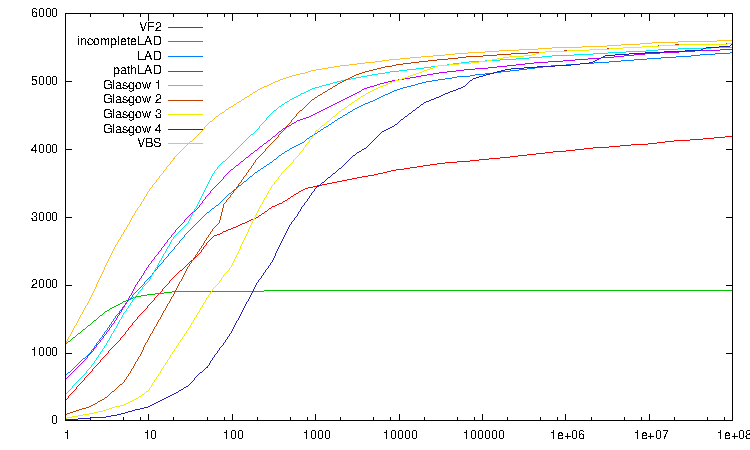
\includegraphics[width=\textwidth]{courbe.pdf}
\caption{Evolution of the number of solved instances with respect to CPU time, for the 8 algorithms of the portfolio, and a Virtual Best Solver (VBS).\label{expTime}}
\end{figure}

\paragraph{Results.}Figure \ref{expTime} displays the evolution of the number of instances solved with respect to CPU time. It shows us that the best solver depends on the time limit
considered. IncompleteLAD is able to solve easy inconsistent instances very quickly, in a few milliseconds. Hence, for time limits lower than 5 ms, the best solver is incompleteLAD. However, it is not able to solve harder inconsistent instances, neither can it solve consistent instances. 

PathLAD and Glasgow(1) outperform incompleteLAD when considering longer time limits: PathLAD is the best solver for time limits larger than 5ms and lower than 40 ms, and Glasgow(1) is the best solver for time limits larger than 40ms and lower than 3000 ms.

Finally, for CPU time limits larger than 3000 ms, the best solver becomes Glasgow(2).
As we increase the CPU time limit, variants of Glasgow with longer paths (Glasgow(3) and Glasgow(4)) become better. This is what we expect, as more reasoning is expensive, but potentially increases the reduction of the search space. In particular, the relative performance of Glasgow variants is monotone in the time it takes to solve the instance – Glasgow(1) is best at first, but gets worse as the time to solve the instance increases until Glasgow(2) is better. After that point, Glasgow(1) is never better than Glasgow(2) again. The same is true for path lengths 3 and 4.

The figure illustrates the potential for portfolios and algorithm selection we have. There is clearly no single solver that dominates throughout.

Furthermore, the Virtual Best Solver (VBS), which considers the best algorithm for each instance
separately, obtains much better results, showing us that the algorithms have complementary
performance. The difference between VBS and single best is more particularly important for rather
small CPU time limits (smaller than 1000 ms). In many applications, it is important to have the
fastest possible algorithm. For example, in pattern recognition applications such as those reported
in \cite{pr15,cviu11}, and in chemical applications such as \cite{Giugno:2013}, we often have to
solve subgraph isomorphism problems for a very large number of graphs (in order to find a pattern
image or molecule in a large database of target images or compounds, for example), so that having an
algorithm that is able to solve an instance in 100 ms instead of 1000 ms makes a big difference.
Therefore, it is important to select the best algorithm for each instance, even if the instance is
an easy one.

Table \ref{expClass} shows us that we cannot reasonably split things up based upon which class instances are coming from, unlike SAT. For all classes, there are always at least 2 algorithms which are the best for at least one instance of the class. In particular, for classes 2 and 3, each algorithm is the best for at least one instance (except Glasgow 4 for Class 3).

\begin{table}[t]
\begin{center}
\begin{tabular}{|c||r||r|r|r||r|r|r|r|}
\hline
Class & VF2 & \multicolumn{3}{c||}{LAD} & \multicolumn{4}{c|}{Glasgow}\\
&&incomplete&default&path&1&2&3&4\\\hline\hline
1 &        0 &       20 &        0 &        0 &       80 &        0 &        0 &        0 \\\hline
2 &      201 &       92 &      189 &      270 &      520 &      180 &       53 &       15 \\\hline
3 &      112 &     1608 &      617 &      959 &      396 &      195 &       21 &        0 \\\hline
4 &      270 &        0 &        0 &        0 &        5 &        0 &        0 &        0 \\\hline
5 &      266 &        0 &        1 &        3 &       31 &        0 &        0 &        0 \\\hline
6 &       71 &        0 &        0 &        0 &        7 &       14 &        1 &        0 \\\hline
7 &      270 &        0 &        0 &        0 &        5 &        0 &        0 &        0 \\\hline
8 &        0 &        0 &        0 &        1 &      195 &       69 &        6 &        0 \\\hline
9 &       77 &        3 &        0 &       19 &      103 &        1 &        0 &        0 \\\hline
10 &       13 &        0 &        2 &        2 &        7 &        0 &        0 &        0 \\\hline
11 &        2 &      142 &       71 &       17 &       23 &        0 &        0 &        0 \\\hline
12 &        0 &        0 &        1 &        2 &      158 &        6 &        1 &        0 \\\hline\hline
Total & 1282 & 1865 & 881 & 1273 & 1530 & 465 & 82& 15\\\hline
\end{tabular}
\end{center}
\caption{Number of times each algorithm is best, for each class.\label{expClass}}
\end{table}

\subsection{Per-Instance Algorithm Selection}

The per-instance algorithm selection problem~\cite{rice_algorithm_1976} is to select from an
algorithm portfolio~\cite{huberman_economics_1997,gomes_algorithm_2001} the one expected to perform
best on a given problem instance. Algorithm selection systems usually build machine learning models
of the algorithms or the portfolio they are contained in to forecast which algorithm to use in a
particular context. Using the model predictions, one or more algorithms from the portfolio are
selected to be run sequentially or in parallel.

Here, we consider the case where exactly one algorithm is selected for solving the problem. One of
the most prominent and successful systems that employs this approach is
SATzilla~\cite{xu_satzilla_2008}, which defined the state of the art in SAT solving for a number of
years. Other application areas include constraint solving~\cite{omahony_using_2008}, the travelling
salesperson problem~\cite{kotthoff_improving_2015}, and AI planning~\cite{seipp_learning_2012}.
The interested reader is referred to a recent survey~\cite{kotthoff_algorithm_2014} for additional
information on algorithm selection.

\medskip

Battiti and Mascia~\cite{battiti-mascia07} were the first to propose
algorithm portfolios for subgraph isomorphism problems. However, they only
consider a pure parallel portfolio without a selection mechanism consisting of
only two solvers. In addition, our instance set is much larger and considers
both hard and unsatisfiable instances.

\section{Algorithm Selection Approach}

Our approach is composed of 3 steps described below. First, we run two presolvers in a static way to
quickly solve easy instances; second, we extract features from instances which are not solved by the
first step; and finally, we select an algorithm and run it.

\subsection{Presolving}

Experimental results reported in Section \ref{expComp} have shown us that incompleteLAD is very fast
(7 ms on average) and is able to very quickly solve 1919 instances. Therefore, we first run
incompleteLAD: if the instance is detected to be unsatisfiable, then we do not process it further.
Otherwise, we record as features the number of candidate couples removed by incompleteLAD in absolute
terms, as a percentage, and the minimum and maximum on a per-variable basis.

VF2 is also able to solve many easy instances very quickly: among the 3806 instances which are not
solved by incompleteLAD, 1470 are solved by VF2 in less than 50 milliseconds. Therefore, after
running incompleteLAD, we run the VF2 solver for 50 ms. This solves easy instances without the
overhead of running algorithm selection and avoids potentially making incorrect solver choices.
After running incompleteLAD and VF2 for 50 ms, we are left with 2336 hard instances that we consider
for algorithm selection.

\subsection{Feature Extraction}

If presolving does not give us a solution, we extract additional features. For both the pattern and
the target graph, we consider some basic graph properties, which may be computed very quickly:

\begin{itemize}
    \item The number of vertices and edges.
    \item The density---we expect that some kinds of filtering might be expensive and ineffective on
        dense graphs.
    \item How many loops (self-adjacent vertices) the graph contains---since loops must be mapped to
        loops, this could have a strong effect on how easy an instance is.
    \item The mean and maximum degrees, and whether or not every vertex has the same degree. (The
        degree-based invariants used by LAD and Glasgow do nothing at the top of search if every
        vertex has the same degree.)
    \item Whether or not the graph is connected.
    \item The mean and maximum distances between all pairs of vertices (if nearly all vertices are
        close together, path-based reasoning is likely to be ineffective). We also consider the
        proportion of vertex pairs which are distance at least 2, 3 and 4 apart.
\end{itemize}

\subsection{Solver Selection}

To decide which solver to run on the remaining instances, we use
LLAMA~\cite{kotthoff_llama_2013}. LLAMA supports the most common algorithm
selection approaches used in the literature. We performed a set of preliminary
experiments to determine the approach that works best in this case.

We use 10-fold cross-validation to determine the performance of the LLAMA
models. The entire set of instances was randomly partitioned into 10 subsets of
approximately equal size. Of the 10 subsets, 9 were combined to form the
training set for the algorithm selection models, which were evaluated on the
remaining subset. This process was repeated 10 times for all possible
combinations of training and test sets. At the end of this process, each problem
instance in the original set was used exactly once to evaluate the performance
of the algorithm selection models.

LLAMA's pairwise regression approach with random forest regression gave the best
performance. The idea is very similar to the pairwise classification used
in~\cite{xu_satzilla_2008}. For each pair of algorithms in our portfolio, we
train a model that predicts the performance difference between them. That is, if
the first algorithm is better than the second, the difference is positive,
otherwise negative. The algorithm with the highest cumulative performance
difference, i.e.\ the most positive difference over all other algorithms, is
chosen to be run.

As this approach gives very good performance already, we did not tune the
parameters of the random forest machine learning algorithm. It is possible that
overall performance can be improved by doing so and we make no claims that the
particular algorithm selection approach we use in this paper cannot be improved.

The data we use in this paper is available as ASlib~\cite{aslib} scenario
GRAPHS-2015.


\section{Experimental Evaluation of Algorithm Selection}

Table~\ref{tab:res} shows the performance of our algorithm selection approach, compared to two
baselines. The virtual best solver is the oracle predictor that, for each instance, chooses the best
solver from our portfolio. This is the upper bound of what an algorithm selection approach can
achieve. The single best solver is the one solver from the portfolio that has the overall best
performance across the entire set of instances, at the CPU time limit of $10^8$ ms, {\em i.e.}, Glasgow(2). We consider it a lower bound on performance.

\begin{table}[ht]
\centering
\begin{tabular}{lr}
  \toprule
& mean runtime\\
  \midrule
virtual best & 5822.809\\
  single best & 7788.719\\
  LLAMA & 6509.947\\
   \bottomrule
\end{tabular}
\vspace{1ex}
\caption{Algorithm selection performance on reduced set of 2336
instances.}\label{tab:res}
\end{table}

We are able to close more than 60\% of the performance gap between the single
best and the virtual best solver, our lower and upper bounds. For comparison, we
show the results achieved on the entire set of instances without
unsatisfiability detection and presolving in Table~\ref{tab:resfull}. We achieve
similar results with more than 58\% of the gap between the single best and the
virtual best closed.

\begin{table}[ht]
\centering
\begin{tabular}{lr}
  \toprule
& mean runtime\\
  \midrule
virtual best & 2375.913\\
  single best & 3177.569\\
  LLAMA & 2706.749\\
   \bottomrule
\end{tabular}
\vspace{1ex}
\caption{Algorithm selection performance on the full set of 5725
instances.}\label{tab:resfull}
\end{table}

Figure~\ref{fig:scatter} shows detailed results for each of the 2336 instances
in the reduced set. Our algorithm selection approach is by no means able to
identify the best solver on a majority of instances, although we are able to
achieve performance improvements overall. There seems to be no particular
pattern as to where algorithm selection performs well and where it fails.

\begin{figure}[!ht]
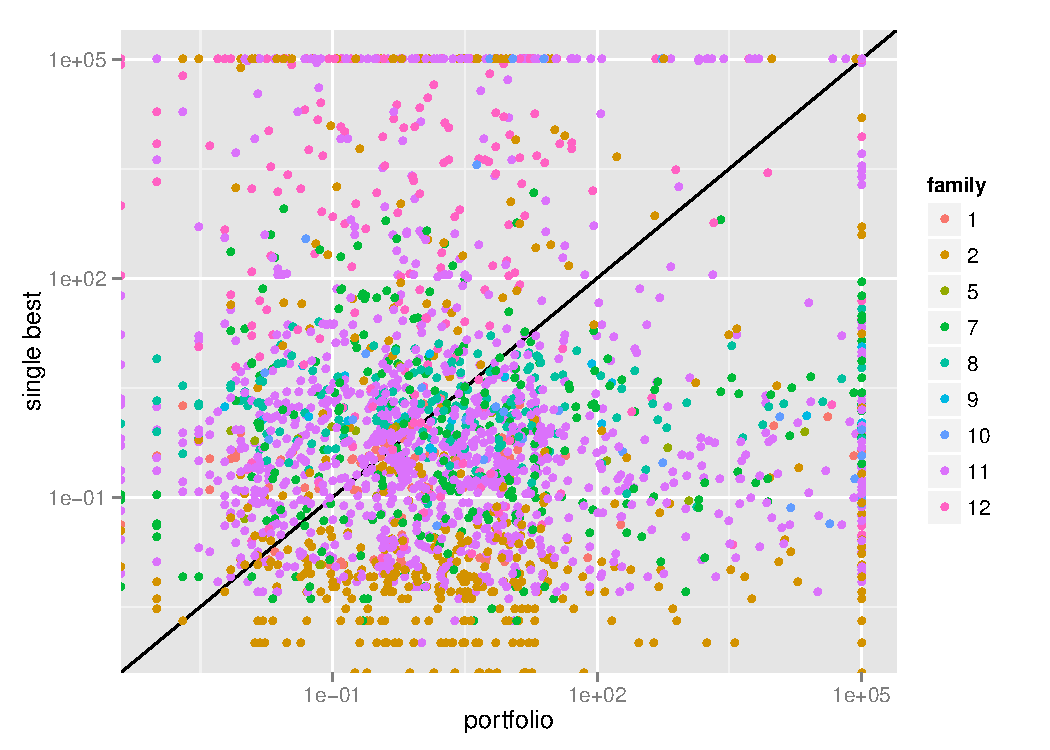
\includegraphics[width=\textwidth]{figures/perfScatter}
\caption{Single best algorithm vs.\ portfolio performance on all instances by
family. Points above the diagonal indicate that the portfolio achieved better
performance, while the single best solver was better on instances below the
diagonal.}
\label{fig:scatter}
\end{figure}

Figure~\ref{fig:portfolio-ecdf} shows the cumulative distribution function for
the individual solvers, the virtual best solver, and the LLAMA portfolio. The
virtual best solver clearly dominates with a significant margin to the next
best. VF2 is far below all other solvers. The portfolio does not perform well
for instances that can be solved quickly because of the overhead incurred
through feature computation. As the instances become more difficult to solve,
its performance improves. For instances that take more than 1,000 seconds to
solve, the portfolio eclipses any individual solver and closes most of the gap
to the virtual best solver.

\begin{figure}[!ht]
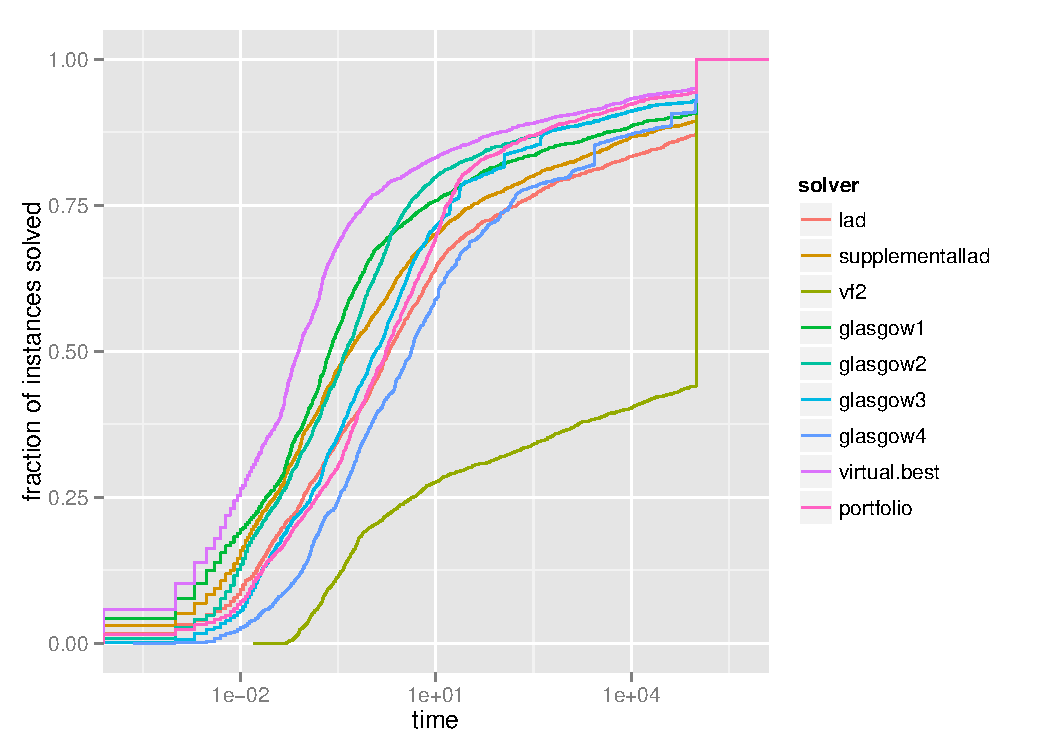
\includegraphics[width=\textwidth]{figures/portfolio-ecdf}
\caption{Empirical cumulative distribution function of solvers, virtual best
solvers, and the LLAMA portfolio.}
\label{fig:portfolio-ecdf}
\end{figure}

\begin{table}[t]
\begin{center}
\begin{tabular}{|c||r||r|r|r||r|r|r|r||r|r|}
\hline
$t$ & VF2 & \multicolumn{3}{c||}{LAD} & \multicolumn{4}{c||}{Glasgow}& VBS & $\delta$\\
&&pre&def&new&1&2&3&4&&\\\hline
$10^0$ & 300 &  \cellcolor{blue!25}1126 & 661 & 599 & 386 & 95 & 39 & 12 & 1132 & 6\\\hline
$10^1$ & 1699 & 1858 & 2101 &  \cellcolor{blue!25}2287 & 2061 & 1215 & 455 & 208 & 3388 & 101\\\hline
$10^2$ & 2834 & 1912 & 3376 & 3708 &  \cellcolor{blue!25}3943 & 3344 & 2295 & 1329 & 4636 & 693\\\hline
$10^3$ & 3458 & 1918 & 4233 & 4531 &  \cellcolor{blue!25}4908 & 4763 & 4262 & 3426 & 5170 & 262\\\hline
$10^4$ & 3701 & 1919 & 4888 & 5025 & 5156 &  \cellcolor{blue!25}5253 & 5022 & 4408 & 5332 & 79\\\hline
$10^5$ & 3850 & 1919 & 5108 & 5193 & 5301 &  \cellcolor{blue!25}5377 & 5292 & 5082 & 5434 & 57\\\hline
$10^6$ & 3977 & 1919 & 5244 & 5307 & 5386 &  \cellcolor{blue!25}5452 & 5451 & 5235 & 5500 & 48\\\hline
$10^7$ & 4082 & 1919 & 5336 & 5414 & 5458 & 5517 &  \cellcolor{blue!25}5518 & 5425 & 5567 & 49\\\hline
$10^8$ & 4191 & 1919 & 5423 & 5479 & 5508 &  \cellcolor{blue!25}5561 & 5560 & 5554 & 5608 & 47\\\hline
\end{tabular}
\end{center}
\caption{Number of solved instances at different CPU time limits: Each line displays a time limit
$t$ (in milliseconds) followed by the number of instances solved within this time limit by VF2, LAD
preprocessing, default LAD, and new LAD, Glasgow with  the lengths of paths limited to 1, 2, 3 and
4, and the VBS. The best single algorithm is highlighted in blue, and the difference between VBS and
single best if displayed in the last column ($\delta$).\label{expTime}}
\end{table}

Table \ref{expTime} displays the number of instances solved at different CPU time limits, ranging
from 1 to $10^8$ milliseconds. It shows us that the best single solver depends on the time limit
considered. Simple approaches like LAD preprocessing and VF2 are able to solve easy instances very
quickly, in a few milliseconds. However, they are not able to solve harder instances: LAD
preprocessing is an incomplete approach which can only detect rather trivial unconsistencies; VF2
performs a basic backtracking search and is very fast on easy instances, because it does not compute
expensive invariants. Default LAD, new LAD, and the Glasgow algorithms solve more instances than VF2
and LAD preprocessing when considering longer time limits: 10 ms for default and new LAD and Glasgow
1, and 100 (resp. 1000 and 10000) ms for Glasgow 2 (resp. 3 and 4). The Virtual Best Solver (VBS),
which considers the best algorithm for each instance separately, obtains much better results,
showing us that the algorithms have complementary performance. The difference between VBS and single
best (column $\delta$ of Table \ref{expTime}) is more particularly important for rather small CPU
time limits. In particular, VBS solves 693 more instances than the single best (Glasgow 1) when the
limit is 100 ms. In many applications, it is important to have the fastest possible algorithm. For
example, in pattern recognition applications, we often have to solve subgraph isomorphism problems
for a very large number of graphs (in order to find a pattern image in a large database of target
images, for example), so that having an algorithm that is able to solve an instance in 100 ms
instead of 1000 ms makes a big difference. Therefore, it is important to select the best algorithm
for each instance.

Table 3 shows the performance of our algorithm selection approach, compared to the VBS (which is the
upper bound of what an algorithm selection approach can achieve), and the single best solver, at
different CPU time limits (the single best corresponds to results highlighted in blue in Table 1).
Comment Table 3: Mean runtime but also number of solved instances at different CPU time limits.
Logically, LLAMA may solve less instances than single best for small time limits because it spends
time to compute features and choose a solver, but it should be better for larger time limits...

\begin{table}
\begin{tabular}{|l|r|rrrrrrrrr|}
&mean & \multicolumn{9}{c|}{Number of solved instances}\\
&runtime & $10^0$ &  $10^1$ &  $10^2$ &  $10^3$ &  $10^4$ &  $10^5$ &  $10^6$ &  $10^7$ &  $10^8$\\\hline
VBS & 2375.9 & 1132 & 3388 & 4636 & 5170 & 5332 & 5434 & 5500 & 5567 & 5608\\\hline
Single best & 3177.6 & 1126 & 2287 & 3943 & 4908 & 5253 & 5377 & 5452 & 5518 & 5561\\\hline
LLAMA & 2706.3\\\hline
\end{tabular}
\caption{}
\end{table}

Add Figure 1 which compares single best at $10^8$ ms (Glasgow 2) with LLAMA ?

\section{Conclusion and Future Work}

Mention parallel, directed, labelled in here briefly.

\bibliographystyle{splncs}
\bibliography{paper}

\end{document}

